\section{Konvektion}
\label{section:convection}
I fasta ämnen går det utmärkt att approximera värmeflöde enbart med hjälp av värmeledningsekvationen. Detta håller dock ej lika bra för fluider, det vill säga material som deformeras då de utsätts för tryck. Under dessa förhållanden måste det tas hänsyn till konservation av massa, rörelsemängd och energi. I det följande kommer en homogen fluid betraktas. För att härleda giltiga differentialekvationer som beskriver en fluids rörelse används ofta sambandet

\begin{equation}
\label{eq:convection:reynolds}
\frac{dB}{dt} = \frac{d}{dt}\left( \int_{V} \frac{dB}{dm} \rho dV \right) + \int_{\partial V} \frac{dB}{dm} \rho \left( \mathbf{v} \cdot \mathbf{n} \right)dA,
\end{equation}

där $B$ är en godtycklig egenskap av fluiden, exempelvis dess rörelsemängd, V är den så kallade kontrollvolymen (omfattande ett godtyckligt valt område), $\partial V$ är denna kontrollvolyms rand, $\rho$ är fluidens densitet, $\mathbf{v}$ är fluidens hastighetsvektor och $\mathbf{n}$ är normalvektorn till randen. Detta samband benämns vanligen Reynolds transportteorem\footnote{För närmare beskrivning och härledning, se White, 2011 \cite{white11}}.

Sätt $B = m$ där $m$ är fluidens massa (oberoende av tiden) och låt $V$ vara en tidsoberoende volym. Ett uttryck för masskonservering erhålls:

\begin{equation}
\label{eq:convection:masscon}
0 = \int_V \frac{\partial \rho}{\partial t} dV + \int_{\partial V} \rho \left( \mathbf{v} \cdot \mathbf{n} \right) dA
\end{equation}

Första termen i detta uttryck beskriver förändringar i densiteten inom kontrollvolymen medan andra termen omfattar alla flöden in och ut genom kontrollvolymens rand. För masskonservering krävs alltså att summan av dessa termer ska vara noll.

Den andra termen kan skrivas om med hjälp av Gauss sat (även kallad divergenssatsen),

\begin{equation}
\label{eq:convection:gauss}
\int_{\partial V} \rho \left( \mathbf{v} \cdot \mathbf{n} \right) dA = \int_V \nabla \cdot \rho \mathbf{v} dV
\end{equation}

\begin{figure}[hpbt]
\centering
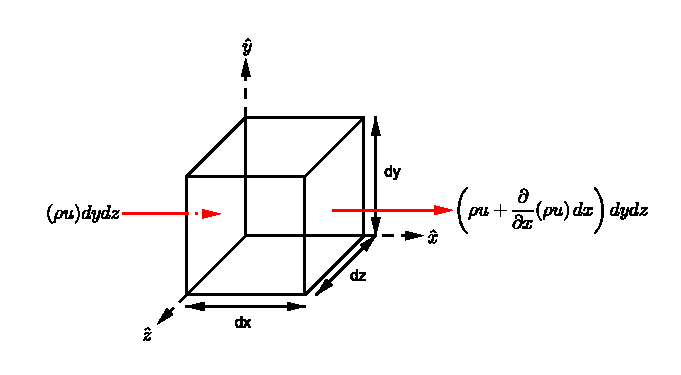
\includegraphics[scale=1]{images/massflowcube.eps}
\caption{\label{fig:massflowcube} Infinitesimal kontrollvolym för derivering av bevaranderelationer, här med massflödet exemplifierat}
\end{figure}

Betrakta nu en infinitesimal kontrollvolym som den i figur \ref{fig:massflowcube}. Integralerna över V ersätts med den infinitesimala volymen $dxdydz$ och \eqref{eq:convection:masscon} reduceras till

\begin{equation}
\label{eq:convection:massconinf}
0 = \left( \frac{\partial \rho}{\partial t} + \nabla \cdot \rho \mathbf{v}\right) dxdydz
\end{equation}

vilket, om $dxdydz$ förkortas bort, kan förenklas som

\begin{equation}
\label{eq:convection:continuity}
\boxed{ \; \; \;
0 = \frac{\partial \rho}{\partial t} + \nabla \cdot \left( \rho \mathbf{v} \right) 
\; \; \; }
\end{equation}

Om inkompressibilitet antas ($\rho$ = konstant) reduceras denna ekvation ytterligare till

\begin{equation}
\label{eq:convection:continuityinc}
\nabla \cdot \mathbf{v} = 0
\end{equation}

Detta är kontinuitetsekvationen för inkompressibla fluider.

Betrakta åter \eqref{eq:convection:reynolds} och sätt nu $B = m\mathbf{v}$. På samma vis som kontinuitetsekvationen \eqref{eq:convection:continuityinc} härleddes, fås för det infinitesimala volymelementet i figur sambandet

\begin{eqnarray}
\label{eq:convection:linear}
\sum \mathbf{F} & = & \frac{\partial}{\partial t} \left( \int_V \rho\mathbf{v} dV \right) + \int_{\partial V} \mathbf{v}\rho\left( \mathbf{v} \cdot \mathbf{n}\right)dV \nonumber \\
& = &\left(\frac{\partial}{\partial t} \left( \rho\mathbf{v} \right) + \nabla \cdot \left( \mathbf{v} \rho \mathbf{v}\right)\right)dxdydz \nonumber\\
& = &\left( \frac{\partial}{\partial t} \left( \rho\mathbf{v} \right) + \mathbf{v}\left(\nabla\cdot\rho\mathbf{v}\right) + \left(\rho\mathbf{v} \cdot \nabla\right) \mathbf{v}\right) dxdydz
\end{eqnarray}

ty enligt Newtons andra lag är tidsderivatan av rörelsemängden $m\mathbf{v}$ lika med summan av alla krafter som verkar på kroppen. $\dot{m}_i$ betecknar här massflödet $\rho\mathbf{v}_i\cdot\mathbf{A}_i$.

Det sista högerledet kan skrivas om som

\begin{equation}
\left( \mathbf{v}\left[ \frac{\partial \rho}{\partial t} + \nabla\cdot \rho \mathbf{v}\right] + \rho\left[ \frac{\partial \mathbf{v}}{\partial t} + u\frac{\partial\mathbf{v}}{\partial x} + v\frac{\partial\mathbf{v}}{\partial y} + w\frac{\partial\mathbf{v}}{\partial z} \right]\right)dxdydz.
\end{equation}

Första termen inom hakparentes är kontinuitetsekvationen \eqref{eq:convection:continuity} och går alltså bort.

Därmed reduceras \eqref{eq:convection:linear} till

\begin{equation}
\label{eq:convection:linearfinal}
\sum \mathbf{F} = \rho \left( \frac{\partial \mathbf{v}}{\partial t} + \mathbf{v}\cdot \nabla\mathbf{v} \right)dxdydz.
\end{equation}

Summan av de på volymen verkande krafterna måste nu utvecklas. Dessa krafter uppstår på grund av gravitation, tryck och viskositet. Andra krafter, såsom från elektromagnetiska fält, kan i sammanhanget anses vara försumbara. Gravitationskraften $\mathbf{F}_g$ beskrivs för den infinitesimala volymen med $\rho \mathbf{g} dxdydz = \rho g dxdydz \hat{z}$. Tryckkraften $\mathbf{F}_p$, i sin tur, ges av tryckgradienten $-\nabla \left( p \right) dxdydz$. Viskösa kraften $\mathbf{F}_{visc}$ är lite besvärligare att sammanställa. Anta att volymen är en Newtonsk fluid, det vill säga stresstensorn $\tau$ är linjärt proportionell mot hastighetsgradienten $\nabla\mathbf{v}$ med proportionaltitetskonstanten $\mu$, $\tau = \mu \nabla \mathbf{v}$. Den viskösa kraften verkande på kroppen blir då $\mathbf{F}_{visc} = \mu\Delta\mathbf{v}dxdydz$.

% Skriv om till integralrelationer och använd gauss sats, därefter infinitesimal volym

Vi har alltså ekvationssystemet

\begin{equation}
\label{eq:convection:momentum}
\addtolength{\fboxsep}{10pt} 
\boxed{ 
\begin{split} 
\rho\left(\frac{\partial u}{\partial t} + \mathbf{v}\cdot \nabla u\right) & = -\frac{\partial p}{\partial x} + \mu\Delta u\\
\rho\left(\frac{\partial v}{\partial t} + \mathbf{v}\cdot \nabla v\right) & = -\frac{\partial p}{\partial y} + \mu\Delta v\\
\rho\left(\frac{\partial w}{\partial t} + \mathbf{v}\cdot \nabla w\right) & = -\rho g -\frac{\partial p}{\partial z} + \mu\Delta w  
\end{split} 
} 
\end{equation}

% Energirelationen

Slutligen sätts i \ref{eq:convection:reynolds} $B=E$ för att söka ett uttryck för energins bevarande. Med antagandet att volymen inte utför något arbete blir $E = Q$, där $Q$ betecknar värmeenergin, och på samma vis som i avsnitt\ref{sec:heatconduction} blir $Q = c_p \rho dT$, vilket ger följande:

\begin{eqnarray}
\label{reynoldsenergyone}
\frac{dQ}{dt} & = & \frac{\partial}{\partial t} \int_V \frac{dQ}{dm}\rho dV + \int_{\partial V}\frac{dQ}{dm}\rho \mathbf{v} \cdot \mathbf{n} dA \nonumber\\
& = & \frac{\partial}{\partial t} \int_V c_p T \rho dV + \int_{\partial V} c_p T \rho \mathbf{v} \cdot \mathbf{n} dA \nonumber\\
& = & \left(\frac{\partial}{\partial t} \left( c_p T \rho \right) + \nabla\cdot c_p T \rho \mathbf{v}\right) dxdydz \nonumber\\
& = & c_p \rho \left( \frac{\partial T}{\partial t} + \mathbf{v}\cdot \nabla T\right)
\end{eqnarray}

Sista steget följer av att kontinuitetsekvationen bryts ut som i fallet med rörelsemängdsekvationen. För att utveckla vänsterledet betraktas återigen en infinetisemal volym såsom i figur \ref{fig:massflowcube}. Värmeenergiflödet in i volymen i x-led ges av $q_x dy dz$ medan utflödet ges av $\left[ q_x + \frac{\partial}{\partial x} \left( q_x\right)dx\right]dydz$ och analogt för y- respektive z-led. Totala ökningen av värmeenergi i kuben ges alltså av utflödet subtraherat från inflödet, vilket innebär att

\begin{equation}
\frac{dQ}{dt} = - \nabla \cdot \mathbf{q} dxdydz.
\end{equation}

$\mathbf{q}$ fås från Fouriers värmelag (se avsnitt \ref{sec:heatconduction}) vilket ger att

\begin{equation}
\label{reynoldsenergytwo}
\frac{dQ}{dt} = \left( - \nabla \cdot \left( -k \nabla T \right) \right)dxdydz
\end{equation}

och detta i sin tur leder till resultatet

\begin{equation}
\label{eq:convection:energy}\boxed{ \; \; \;
\nabla \cdot \left( k \nabla T \right) = c_p \rho \left( \frac{\partial T}{\partial t} + \mathbf{v}\cdot \nabla T\right)
\; \; \;}
\end{equation}

För homogena inkompressibla fluider i två dimensioner gäller alltså ekvationerna
\eqref{eq:convection:continuityinc}, \eqref{eq:convection:momentum} samt \eqref{eq:convection:energy}.

\subsection{Vindens konvektionskoefficient}

Då vinden blåser kommer en del värmeenergi överföras via konvektion, men istället för att lösa den invecklade konvektions-diffussionsekvationen används ofta något som kallas för vindens konvektionskoefficient, betecknat med $h$. I analogi med Fouriers värmelag, ekvation \ref{eq:conduction:fourier}, skrivs

\begin{equation}\boxed{ \; \; \;
q = hdT = h\left( T_{wall} - T_{\infty}\right).
\; \; \;}\end{equation}

där h alltså ka jämföras med det ovan härledda U-värdet. 

Denna konvektionskoefficient beskrivs ofta av en ekvation anpassad till empiriska resultat, och ett stort antal experiment har genomförts för att bestämma parametern, även om en helhetsbild saknas i dagsläget.

Vid fri (naturlig) konvektion, det vill säga då vinden är försumbar och luftcirkulationen följer av stigande varm luft, brukar h fås till mellan 2 och $\unit{25}{Wm^{-2}K^{-2}}$. Vid forcerad konduktion, det vill säga då vinden inte är försumbar, kan h variera från 25 till $\unit{250}{Wm^{-2}K^{-2}}$. \cite{ASHRAE09}

Traditionellt används ofta något som kallas för Nusselt-Jürges korrelation vid beräkning av konvektionskoefficienten, som lyder

\begin{equation}
h = 5.678 \left( a + b \left( \frac{965.42}{T_{out}}\left(|\mathbf{v}_{wind}\times \mathbf{n}|\right) \right)^c \right)
\end{equation}

där $\mathbf{n}$ betecknar väggens normalvektor, och a, b samt c beror på väggens ytegenskaper. För en skrovlig yta med $|\mathbf{v}_{vind}\times \mathbf{n}| < \unit{4.88}{ms^{-1}}$ fås att $a=1.09$, $b=0.23$ samt $c=1$, medan starkare vind ger $a=0$, $b=0.53$ samt $c=0.78$.

En mängd andra samband mellan konvektionskoefficienten och vindhastigheten har härletts, både teoritiskt och empiriskt, på grund av dess starka beroende av byggnadens ytegenskaper och area, men av anledningar som diskuteras i avsnitt \ref{sec:errors}.\cite{palyvos08}

% Skapa graf över T och v beroende

\subsection{Boussinesq approximation}

För flytkraftsdrivet flöde kan det vara lämpligt att använda sig av
Boussinesq approximation. Denna säger att det enda som påverkar trycket är
tyngdaccelerationen. Genom detta är det möjligt att sätta upp uttryck för densiteten
och tryckderivatorna enligt ekvationerna \eqref{eq:convection:density}
och \eqref{eq:convection:pressurez}. Här är
$\beta$ den volymetriska expansionskonstanten och
$T_0$ temperaturen som råder vid referensdensiteten $\rho_0$.

\begin{equation}
\label{eq:convection:density}
\rho = \rho_0[1-\beta(T-T_0)]
\end{equation}

\begin{equation}
\label{eq:convection:pressurez}
\frac{\partial p}{\partial z} = -\rho_0g
\end{equation}


